Mathematicians are often skeptical of proofs backed by extensive computation.
A landmark example is the \emph{four-color theorem}, which states that any planar graph can be colored with at most four colors. 
In 1879, Alfred Kempe published a proof of the four-color theorem, which was discovered to be incorrect 11 years later by Headwood~\cite{Walters2004ItAT,Wilson2002GraphsCA}.\footnote{The main idea of Kempe's proof was salvaged by Headwood to prove the weaker \emph{five-color theorem}, and it is still a building block in the theory of planar colorings~\cite{Walters2004ItAT}.} 
A full proof of the four-color theorem was not found until 1976, when Kenneth Appel and Wolfgang Haken used a computer to verify the 1\,834 cases that provably could contain a counterexample~\cite{appelFourColorProblem1978}.
Their proof was controversial, and indeed, small errors have been found in their initial calculations~\cite{Walters2004ItAT,Wilson2002GraphsCA}.
Finally, in 2005, Georges Gonthier formalized a full proof of the four-color theorem in the \textsf{Coq} proof assistant~\cite{gonthierFourColourTheorem2008a}, thus laying to rest any lingering doubts about the correctness of the result. To the best of our knowledge, all proofs known for this theorem require the assistance of computers.

Nevertheless, the four-color theorem is far from the end of the story when it comes to computationally proven theorems.
In particular, an emerging trend in computer-assisted mathematics is to use SAT solvers (or more in general, automated reasoning tools), to prove mathematical theorems by analyzing finite objects~\cite{avigad2023mathematics}. 
To name a few examples,  Erd\H{o}s Discrepancy Conjecture~\cite{konev2014sat}, Keller's conjecture~\cite{brakensiek2023resolution}, the Packing Chromatic number of the infinite grid~\cite{Subercaseaux_Heule_2023}, and the Pythagorean Triples Problem~\cite{Heule_2016} have all been solved using SAT solvers.
All such SAT-based results follow a common structure; in order to show that a mathematical theorem $\mathcal{T}$, potentially regarding infinite objects, holds, one proves the following:
\begin{enumerate}
  \item (\textbf{Reduction Theorem}) There is a finite object $\mathcal{O}$ such that either (\emph{positive case}) $\mathcal{T}$ holds if and only if $\mathcal{O}$ exists, or (\emph{negative case}) $\mathcal{T}$ holds if and only if $\mathcal{O}$ does not exist.
  \item (\textbf{Encoding Theorem}) There is a CNF formula $\varphi_{\mathcal{O}}$ that is satisfiable if and only if $\mathcal{O}$ exists.
  \item (\textbf{SAT Result}) In the \emph{positive case}, a SAT solver finds a satisfying assignment for $\varphi_{\mathcal{O}}$, and in the \emph{negative case}, a SAT solver finds that $\varphi_{\mathcal{O}}$ is unsatisfiable.
\end{enumerate}
To complicate things further, the formula $\varphi_{\mathcal{O}}$ that directly encodes the existence of the desired object $\mathcal{O}$ is often too large or computationally hard to be solved directly, and therefore it is necessary to obtain an easier formula $\phi_{\mathcal{O}}$ that is equisatisfiable to $\varphi_{\mathcal{O}}$, thus requiring as well a ``\textbf{Reencoding Theorem}''. This is the case for all the aforementioned problems, and also for the Empty Hexagon theorem at the heart of this article. 
In the \emph{positive case} for the SAT result, it is usually possible to directly reconstruct the desired object $\mathcal{O}$ from a satisfying assignment of $\phi_{\mathcal{O}}$, and then by directly exhibiting $\mathcal{O}$, the correctness of theorem $\mathcal{T}$ can be easily verified by humans. The \emph{negative case} is however much harder, as the unsatisfiable proofs emitted by SAT solvers can be inhumanly large. For example, the resolution of the Boolean Pythagorean triples problem required an unsatisfiability proof of 200 terabytes, the largest known to date~\cite{Heule_2016,lambTwohundredterabyteMathsProof2016}.
This raises a fundamental question for computational mathematics:
\begin{center}
  \emph{How can we trust the correctness of a theorem $\mathcal{T}$ that has been proven through a very long unsatisfiability proof?}
\end{center}
\begin{figure}[ht]
    \centering
    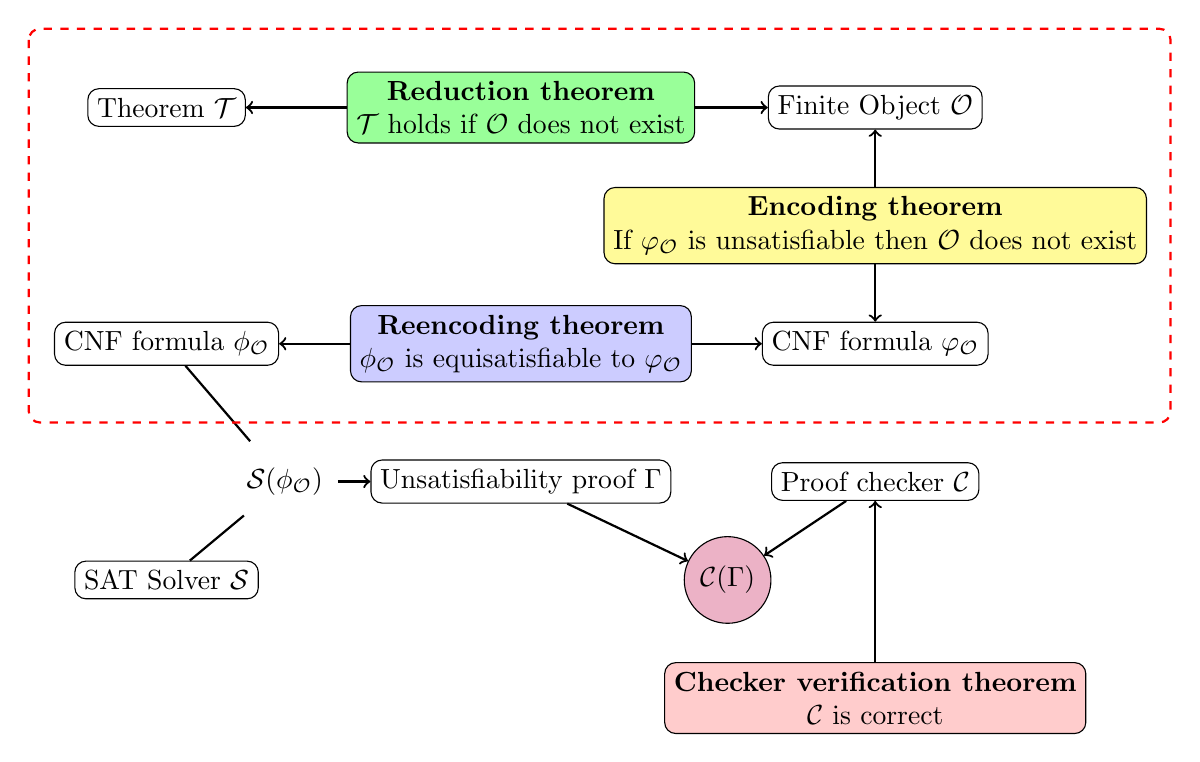
\begin{tikzpicture}
      \node[draw, rounded corners] (theorem) at (0,0) {Theorem $\mathcal{T}$};
      \node[draw, rounded corners] (object) at (9,0) { Finite Object $\mathcal{O}$};
      \node[draw, rounded corners, align=center, fill=green!40!white] (tiffo) at (4.5,0) { \textbf{Reduction theorem}\\$\mathcal{T}$ holds if $\mathcal{O}$ does not exist};
      \draw[->, thick] (tiffo) -- (theorem);
      \draw[->, thick] (tiffo) -- (object);
      \node[draw, rounded corners, align=center] (varphi) at (9, -3) {CNF formula $\varphi_{\mathcal{O}}$};
      \node[draw, rounded corners, align=center, fill=yellow!40!white] (encoding) at (9, -1.5) { \textbf{Encoding theorem}\\If $\varphi_{\mathcal{O}}$ is unsatisfiable then $\mathcal{O}$ does not exist};
      \draw[->, thick] (encoding) -- (object);
      \draw[->, thick] (encoding) -- (varphi);
      \node[draw, rounded corners] (phi) at (0, -3) {CNF formula $\phi_{\mathcal{O}}$};
      \node[draw, rounded corners, align=center, fill=blue!20!white] (equisat) at (4.5, -3) { \textbf{Reencoding theorem}\\$\phi_{\mathcal{O}}$ is equisatisfiable to $\varphi_{\mathcal{O}}$};
      \draw[->, thick] (equisat) -- (phi);
      \draw[->, thick] (equisat) -- (varphi);
      \node[draw, rounded corners] (solver) at (0, -6) {SAT Solver $\mathcal{S}$};
      \node[draw, rounded corners] (unsat-proof) at (4.5, -4.75) {Unsatisfiability proof $\Gamma$};
      \node[circle] (solverphi) at (1.5, -4.75) {$\mathcal{S}(\phi_{\mathcal{O}})$};
      \draw[-, thick] (solver) -- (solverphi);
      \draw[-, thick] (phi) -- (solverphi);
      \draw[->, thick] (solverphi) -- (unsat-proof);
      \node[draw, rounded corners] (checker) at (9, -4.75) {Proof checker $\mathcal{C}$};
      \node[circle, draw, fill=purple!30!white] (checkerphi) at (7.125, -6) {$\mathcal{C}(\Gamma)$};
      \draw[->, thick] (unsat-proof) -- (checkerphi);
      \draw[->, thick] (checker) -- (checkerphi);
      \node[draw, rounded corners, align=center, fill=red!20!white] (checkerCorrectness) at (9, -7.5) { \textbf{Checker verification theorem}\\$\mathcal{C}$ is correct};
  
      \draw[->, thick] (checkerCorrectness) -- (checker);
      \draw[red, dashed, thick, rounded corners] (-1.75,1) -- (-1.75, -4) -- (12.75, -4) -- (12.75, 1) -- cycle;
    \end{tikzpicture}
    \caption{General structure of the verification pipeline for a SAT-based theorem in the \emph{negative case}. The dashed rectangle encloses the main focus of this paper, whereas for the rest of the proof we leverage already existing tools.}\label{fig:proof-structure}
  \end{figure}
The main contribution of this article is to provide the first example of a formally verified proof of such a theorem, thus addressing the question above.
The pipeline required for such a verified proof involves several components, as illustrated in~\Cref{fig:proof-structure}, and each of them will be detailed in the rest of the paper.

\paragraph{The Empty Hexagon Number.}
In the 1930s, Stein, Erd\H{o}s and Szekeres kickstarted a geometric turn for Ramsey theory by studying how many points in the plane in \emph{general position} (i.e., no three points on a common line) are required for a convex $k$-gon to always appear. Let $g(k)$ be the minimum number $n$ such that any $n$ points in general position are guaranteed to contain a convex $k$-gon. Then, the celebrated Erd\H{o}s-Szekeres theorem states that $g(k) \leq \binom{2k-4}{k-2} + 1$~\cite{erdosCombinatorialProblemGeometry2009}. Moreover, Erd\H{o}s and Szekeres conjectured that $g(k) = 2^{k-2} + 1$, which has only been proven for $k \leq 6$. In a similar spirit, Erd\H{o}s defined $h(k)$ as the minimum number of points in general position that is guaranteed to contain a $k$-hole (i.e., a convex $k$-gon without any other point inside).
It is easy to check that $h(3) = 3$ and $h(4) = 5$. In 1978, Harborth established that $h(5) = 10$~\cite{Harborth1978}, and in a surprising turn of events, Horton proved in 1983 that $h(7) = \infty$, meaning one could always avoid $7$-holes~\cite{hortonSetsNoEmpty1983}. 
The only case left open was thus $h(6)$. The \emph{Empty Hexagon Theorem}, proven independently by Gerken and Nicolás in 2006, and then refined by Valtr in 2008, established that $h(6)$ was finite. 
However, the resulting best bounds presented a wide gap, as it was only known that $29 \leq h(6) \leq 1717$. In a recent breakthrough, Heule and Scheucher used a SAT solver to prove that $h(6) = 30$~\cite{emptyHexagonNumber}, a result we refer to as \emph{``The Empty Hexagon Number''}. Now that all values of $h$ are now known, and especially given the extensive computation involved in their proofs, we believe that the formal verification of the Empty Hexagon Number represents a crucial step towards the full resolution of the area of research initiated by Stein, Erd\H{o}s, and Szekeres almost a century ago.

\paragraph{Outline of the paper.} \Cref{sec:triple-orientations} discusses the basic geoemtric aspects of the problem, and in particular, \emph{triple orientations} (also known as \emph{signotopes}), a fundamental tool in computational geometry to represent discretely problems involving an a priori continuous space (i.e., $\mathbb{R}^2$), which is the basis of Heule and Scheucher's SAT encoding. Then,~\Cref{sec:symmetry-breaking} deals with two assumptions that are key to break symmetries in the problem and thus make the SAT encoding practically feasible. Namely, that one can assume without loss of generality the following two properties at the same time: (i) points are labeled from left to right without two of them having the same $x$-coordinate, and (ii) the triples $(p_1, p_i, p_j)$ are always oriented counterclockwise for $i < j$. 
\Cref{sec:leansat} presents the \emph{LeanSAT} library, which plays a key role in proving the correctness of encodings. Next,~\Cref{sec:empty-triangle} presents how the previous elements are already enough to formalize a SAT-based proof for the \emph{Empty Triangle Theorem}, a much simpler variant involving only triangles that does not require reencodings. \Cref{sec:empty-hexagon-number} presents the details of the formalization of $h(6) = 30$, the Empty Hexagon Number. We conclude by discussing the next steps towards the formal verification of other Erd\H{o}s-Szekeres-type problems.
